\textbf{It is tempting to bring a list of technologies out as a glorious
cookbook.} We need a 1/2 cup of group writing tools, 2 tsp. of social
network elements, a thick slice of social bookmarking, and some sugar,
then put it in the oven for 1 hour for 350 degrees.

We have created a broad features/functions list for Handbook readers to
reflect upon and consider. The joy of this list is that you can consider
alternatives for the way you communicate and work while you are planning
the project, or can add in new elements to solve communications gaps or
create new tools.

However, too many tools spoil the broth. In the writing of this
Handbook, we found that out firsthand. We spent a lot of marvelous
energy exploring different tools to collaborate, curate information, do
research, tag resources, and adjudicate among all of our points of view.
In looking at groups working with the various MOOCs, as another example,
different groups of students often camp in different social media
technologies to work. In large courses, students often have to be pushed
into various social media tools to ``co-create'' with great protest and
lots of inertia. And finally, co-learning groups often come from very
different backgrounds, ages, and stages of life, with very different
tools embedded in their current lives. Do we have time for three more
tools in our busy days? Do more tools help or interfere in our work?

In this section, we'll share with you a few issues:

\begin{itemize}
\item
  What technologies are most useful in peer learning? What do we use
  them for? What features or functions help our co-learning process?
\end{itemize}
\begin{itemize}
\item
  How do we decide (a) as a group and (b) for the group on what tools we
  can use? Do we decide upfront, or grow as we go?
\end{itemize}
\begin{itemize}
\item
  How do we coach and scaffold each other on use of tools?
\end{itemize}
\begin{itemize}
\item
  How much do the tool choices impact the actual outcome of our learning
  project?
\end{itemize}
\begin{itemize}
\item
  What are the different roles that co-learners can take in co-teaching
  and co-coaching the technology affordances/assumptions in the project
  to make others' lives easier?
\end{itemize}
\subsection{Features and Considerations}

We will begin below with a discussions of ``features'' and initial
considerations, and then move to a broader ``Choose Your Own
Adventure''-style matrix of features leading to a wide variety of
collaboration-based technology tools online.

\subsubsection{Technologies and Features}

As we will share in the extensive list below, there are abundant tools
now available -- both for free and for pay -- to bring great features to
our co-learning endeavors. It is tempting to grab a group of fancy tools
and bring the group into a fairly complex tool environment to find the
perfect combination of resources. The challenge: as Adult Learners, we
seek both comfort and context in our lives (Schein,
\href{\#schein97}{1997}, \href{\#schein04}{2004}). In choosing tools as
Brands and technologies, we can ignore the features themselves and what
we need as parts of the puzzle for learning. We also can have anxiety
about our self-beliefs around computers and technology, which in turn
can limit our abilities \href{\#compeau}{(Compeau \& Higgins, 1995)}.

Before we get to Brands and choices, it helps to ask a few questions
about the learning goals and environments:

\begin{itemize}
\item
  What do we need as features, and at what stage of the learning
  process?
\item
  What are we already comfortable with, individually and as a group?
\item
  Do we want to stay with comfortable existing tools, or do we want to
  stretch, or both?
\item
  What types of learners do we have in this group? Technologically
  advanced? Comfortable with basics?
\item
  Do we want to invest the time to bring the whole group up to speed on
  tools? Do all the group members agree on this? Do we want to risk
  alienating members by making them invest time in new resources?
\item
  We know that our use will migrate and adapt. Do we want to plan for
  adaptation? Observe it? Learn from it? Make that change intentional as
  we go?
\end{itemize}
Researchers over the years have heavily examined these questions of
human, technology, and task fit in many arenas.
\href{http://en.wikipedia.org/wiki/Human-Computer\_Interaction}{Human-Computer
Interaction} researchers have looked at ``fit'' and ``adaptive
behavior,'' as well as how the tools can affect how the problem is
presented in the work \href{\#teeni}{(Te'eni, 2006)}. Creativity support
tools \href{\#shneiderman}{(Shneiderman, 2002)} have a whole line of
design research, as has the field of
\href{http://en.wikipedia.org/wiki/Computer-supported\_cooperative\_work}{Computer-Supported
Collaborative Work Systems (CSCW)}. For co-learners and designers
interested in the abundance in this space, we've added some additional
links below.

We here will make this a bit easier. For your co-learning environment,
you may want to do one or two exercises in your decision planning:

\begin{itemize}
\item
  What \textbf{features do you need}? Do you need collaboration? Graphic
  models? Places to work at the same time (synchronous)? Between
  meetings (asynchroous)?
\item
  What are the group members \textbf{already using} as their personal
  learning platforms? It also makes sense to do an inventory about what
  the group already has as their learning platforms. I'm doing that with
  another learning group right now. People are much more comfortable --
  as we also have found in our co-creation of this Handbook -- creating
  and co-learning in tools with which they already are comfortable.
  Members can be co-teachers to each other -- as we have have -- in new
  platforms.
\item
  What \textbf{type of tools}, based on the features that we need, shall
  we start out with? \href{\#resnick}{Resnick at al. (2005)}looked at
  technology tools having
  \begin{itemize}
  \item
    Low thresholds (easy to get people started)
  \item
    Wide walls (able to bring in lots of different situations and uses)
    and
  \item
    High ceilings (able to do complex tasks as the users and uses adapt
    and grow).
  \end{itemize}
\end{itemize}
What are important features needed for co-creation and \textbf{working
together}? In other pages above, we talk abundantly about roles and
co-learning challenges. These issues also are not new;
\href{\#dourish}{Dourish \& Bellottii back in 1992} for example, shared
long-standing issues in computer-supportive collaborative work online
about how we are aware of the information from others, passive vs.
active generation of information about collaborators, etc. These
challenges used to be ``solved'' by software designers in individual
tools. Now that tools are open, abundant, and diverse, groups embrace
these same challenges when choosing between online resources for
co-learning.

Which of these will be important to your group work? Keep in mind --
your needs for tools, plus how the group uses them, \emph{\textbf{will
change as the co-learning project moves along}}. Are you willing to
change tools during the project as your needs and users change, or do
you want to plan on tools that are great in all these dimensions at the
start?

\subsubsection{Useful Uses and fancy Features of Technological Tools}

From here, we will help you think about what might be possible, linking
to features and solution ideas.

We start with ways to ask the key questions: What do you want to do and
why? We will start with features organized around several different
axes:

\begin{itemize}
\item
  \href{\#time-place}{Time/Place}
\item
  \href{\#stages}{Stages of Activities and Tasks}
\item
  \href{\#skill}{Skill Building/Bloom's Taxonomy}
\item
  \href{\#use}{Use Cases}, and
\item
  \href{\#functions}{Learning Functions}.
\end{itemize}
Each will link to pages that will prompt you with features,
functionality, and technology tool ideas.

\subsubsection{Time/Place}

We can further break down tools into whether they create or distribute,
or whether we can work simultaneously (synchronous) or at our own times
(ascynchronous). To make elements of time and place more visual,
\href{\#baeker}{Baecker (1995)} created a CSCW Matrix, bringing together
time and place functions and needs:

\ctable[pos = H, center, botcap]{p{.3\textwidth}p{.3\textwidth}p{.3\textwidth}}
{% notes
}
{% rows
\FL
&\shifttext{-4mm}{\begin{tabular}{l}
\textbf{Same Time} \\
\textbf{(Synchronous)}
\end{tabular}}
&\shifttext{-4mm}{\begin{tabular}{l}
\textbf{Different Time} \\
\textbf{(Ascynronous)}
\end{tabular}}
\\ \noalign{\medskip}
\raisebox{-4mm}
{\begin{tabular}{l}
\textbf{Same Place} \\
\textbf{(Colocated)}
\end{tabular}} & \textbf{Face-to-Face}:
Display-focused (e.g., Smartboards) 
& \textbf{Continuous Task}:
Groupware, project management
\\\noalign{\medskip}
\raisebox{-4mm}{\begin{tabular}{l}
\textbf{Different Place} \\
\textbf{(Remote)}
\end{tabular}} & \textbf{Remote Interaction}:
Videoconference, IM, Chat, Virtual Worlds & \textbf{Communication \&
Coordination}: Email, bulletin boards, Wikis, blog, workflow tools
\LL
}

Some tools are synchronous, such as Google+ Hangouts, Blackboard
Collaborate, and Adobe Connect, while others let us work asynchronously,
such as wikis, forums, and Google Docs. We seem to be considering here
mostly tools good for group work, but not for solo, while many others
are much easier solo or in smaller groups.

\subsubsection{Stages of Activities and Tasks}

\href{\#shneiderman}{Dan Shneiderman} (2002) has simplified the abundant
models in this area (e.g., Couger and Cave) with a clear model of 4
general activities and 8 tasks in creation for individuals, which we can
lean on as another framework for co-creation in co-learning.

\subsection{\textbf{Activities}}

\subsection{\textbf{Tasks}}

\subsection{Collect}

\begin{itemize}
\item
  Searching
\item
  Visualizing
\end{itemize}
\subsection{Relate}

\begin{itemize}
\item
  Consulting Others
\end{itemize}
\subsection{Create}

\begin{itemize}
\item
  Thinking (Free Association)
\item
  Exploring
\item
  Composing
\item
  Reviewing
\end{itemize}
\subsection{Distribute}

\begin{itemize}
\item
  Disseminating
\end{itemize}
Tools and functions won't be clear cut between areas. For example, some
tools are more focused on being generative, or for creating content.
Wikis, Etherpad, Google docs, and others usually have a commenting/talk
page element, yet generating content is the primary goal and
discursive/consultative functions are in service of that. Some tools are
discursive, or focused on working together for the creative element of
``relating'' above -- Blackboard Collaborate, the social media class
room forums, etc.

\subsubsection{Skill Building (Cognitive, a la Bloom's Taxonomy, see
below)}

Given that we are exploring learning, we can look to Bloom's Taxonomy
(revised, \href{\#anderson}{Anderson \& Krathwohl, 2001}) for guidance
as to how we can look at knowledge support. Starting at the bottom, we
have:

\begin{itemize}
\item
  Remembering, as a base;
\end{itemize}
\begin{itemize}
\item
  Understanding,
\end{itemize}
\begin{itemize}
\item
  Applying,
\end{itemize}
\begin{itemize}
\item
  Analyzing,
\end{itemize}
\begin{itemize}
\item
  Evaluating, and then, at the top,
\end{itemize}
\begin{itemize}
\item
  Creating.
\end{itemize}
We could put ``search'' in the Remembering category above. Others
{[}need to re-find and cite{]} contest that Search, done well, embraces
most of the Bloom's elements above. Samantha Penney has created a
Bloom´s Digital Taxonomy Pyramid of tools for learning (cc 3.0 --
\href{http://www.usi.edu/distance/bdt.htm)}{http://www.usi.edu/distance/bdt.htm)}.

\begin{figure}[htbp]
\centering
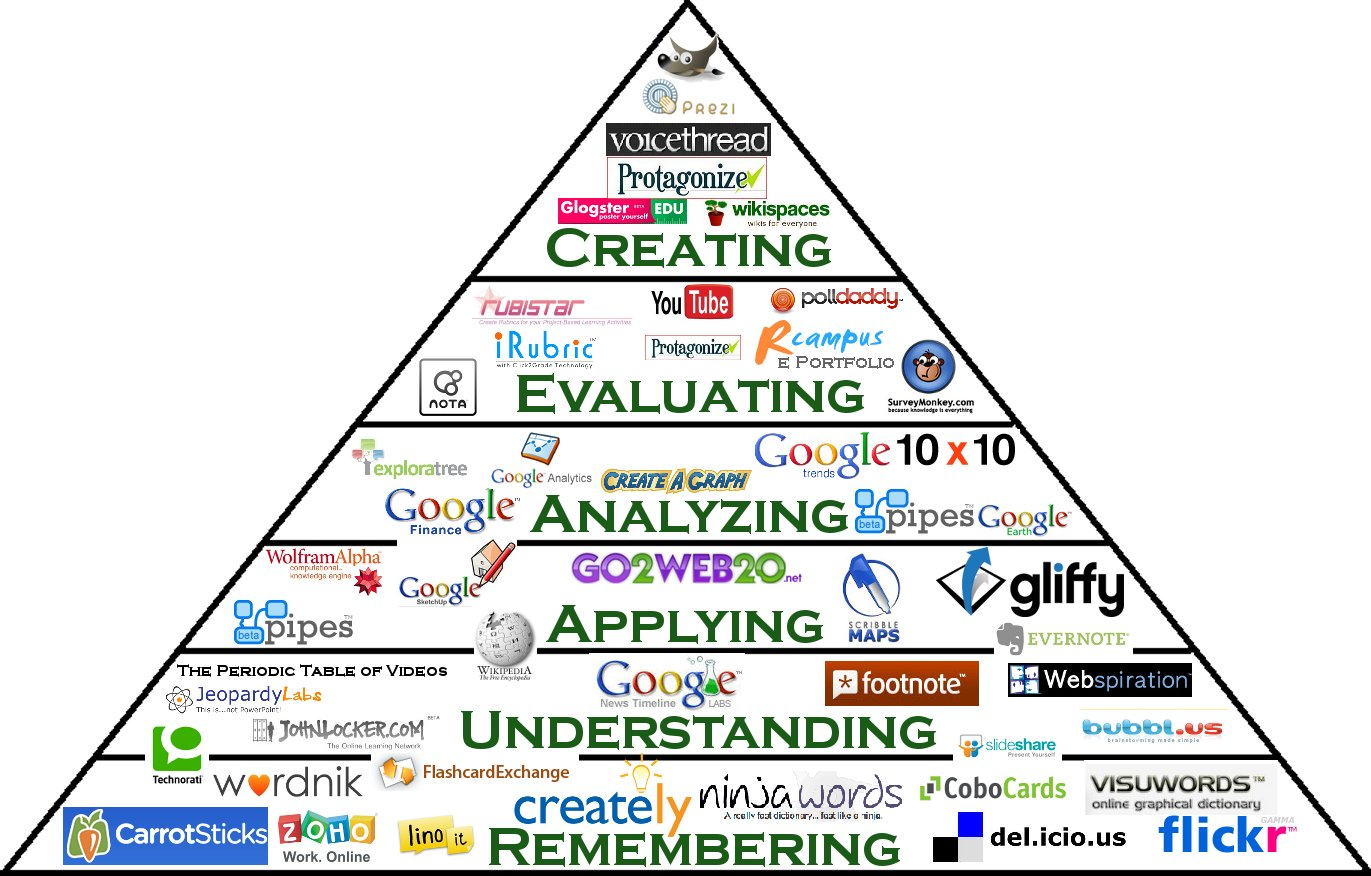
\includegraphics[width=.65\textwidth]{../pictures/blooms.jpg}
\end{figure}

\subsubsection{Use Cases (I want to\ldots{}.)}

Technologies can be outlined according to the need they serve or use
case they fulfill. Examples: If we need to `curate', Pearl Trees is an
option. To `publish' or `create', we can look to a wiki or wordpress.
Other choices might be great in order to `collaborate', etc.

One challenge is that tools are not that simple. As we look more closely
at the technologies today, we need to reach more broadly to add multiple
tags to them. For example Twitter can be used for ``Convening a group,''
for ``micro-blogging,'' for ``research,'' etc.

\begin{itemize}
\item
  Collaborate with a Group
\end{itemize}
\begin{itemize}
\item
  Create Community
\end{itemize}
\begin{itemize}
\item
  Curate Information (select content, contextualize, and share it)
\end{itemize}
\begin{itemize}
\item
  Research
\end{itemize}
\begin{itemize}
\item
  Publish Information
\end{itemize}
\begin{itemize}
\item
  Create Learning Activities
\end{itemize}
\begin{itemize}
\item
  Make Something
\end{itemize}
These plans get more complex, as you are making a group of decisions
about tool functionality in order to choose what combination works for
use cases. It may be most useful to use a concept map (a tech tool) to
think about the needs and combinations that you would bring together to
achieve each Use Case or Learning Module.

\subsubsection{Technology Features/Functions}

We have not made this easy! There are lots of moving elements and
options here, none of them right for everything, and some of them
fabulous for specific functions and needs. Some have the low thresholds
but may not be broad in scope. Some are broad for many uses; others are
specific task-oriented tools. That is some of the charm and frustration.

Weaving all of the above together, we have brought together a shared
taxonomy for us to discuss and think about co-learning technology
features and functions, which we present as an appendix below. This
connects various technology features within an expanded version of Ben
Shneiderman's creativity support tools framework. We've created this
linked toolset with multiple tags, hopefully making it easier for you to
evaluate which tool suits best the necessities of the group. Please
consider this a starting point for your own connected exploration.

\subsection{Appendix: Features and Functions}

Weaving all of these frameworks together, we have brought together a
shared taxonomy for us to discuss and think about co-learning technology
features and functions. We have connected various technology features
with an expanded version of Ben Shneiderman's creativity support tools
framework for the linked resource guide.

Note: please add tools as posts that follow the following
\href{http://peeragogy.org/tool-post-template/\%20?}{template} format.

\emph{\textbf{Click the links below}} to take you to samples of each of
these features and functions in groups of tools. Please consider this a
starting point for your own connected exploration.

\textbf{Activities}

\textbf{Tasks}

\textbf{Features/Functions}

\subsection{Planning/Designing (a cycle of Learning before the
Co-Learning)}

\begin{itemize}
\item
  Communicating
\item
  Deciding and Creating Alternatives
\end{itemize}
\begin{itemize}
\item
  \href{http://peeragogy.org/convening-group/}{Convening a group}
\item
  \href{http://peeragogy.org/planning-a-coursestructure/}{Planning a
  course/structure}
  \begin{itemize}
  \item
    Assembling a syllabus
  \end{itemize}
  \begin{itemize}
  \item
    Designing a learning activity
  \end{itemize}
\item
  \href{http://peeragogy.org/designing-self-assessment/}{Designing
  self-assessment} (group and individual)
\item
  \href{http://peeragogy.org/setting-goals/}{Setting individual and
  group goals}
\item
  \href{http://peeragogy.org/brainstorming/}{Brainstorming}
\item
  \href{http://peeragogy.org/visualizing/}{Visualizing}
\end{itemize}
\subsection{Collect/Share Inbound}

\begin{itemize}
\item
  Searching
\item
  Visualizing
\end{itemize}
\begin{itemize}
\item
  \href{http://peeragogy.org/search/}{Search}
\item
  \href{http://peeragogy.org/social-bookmarking/}{Social Bookmarking}
\item
  \href{http://peeragogy.org/taxonomics/}{Creating/Finding Taxonomies}
  (shared keywords, domain-based keywords)
\item
  \href{http://peeragogy.org/programming-toolsets/}{Programming
  Toolsets}
\item
  \href{http://peeragogy.org/collaborative-reading/}{Collaborative
  reading}
\item
  \href{http://peeragogy.org/collaborative-note-taking/}{Collaborative
  note-taking}
\item
  \href{http://peeragogy.org/curation-tools/}{Curation Tools}
\item
  \href{http://peeragogy.org/recording-information-inputs/}{Gathering
  information} (e.g., capturing audio, video, text)
\item
  \href{http://peeragogy.org/surveys-and-questionnaires/}{Surveys and
  Questionnaires}
\end{itemize}
\subsection{Relate}

\begin{itemize}
\item
  Consulting Others from the Outside
\end{itemize}
\begin{itemize}
\item
  \href{http://peeragogy.org/qualitative-research/}{Qualitative
  research}
\item
  \href{http://peeragogy.org/quantitative-research/}{Quantitative
  research}
\end{itemize}
\subsection{Communication}

\begin{itemize}
\item
  Connecting with Others in the Group
\end{itemize}
\begin{itemize}
\item
  \href{http://peeragogy.org/planning-and-scheduling/}{Project Planning
  - Scheduling}
\item
  \href{http://peeragogy.org/voice-and-video-conferencing/}{Voice/Video
  Conferencing Services}
\item
  \href{http://peeragogy.org/group-communication/}{Group Email / Forum
  Messaging Services}
\item
  \href{http://peeragogy.org/file-sharing/}{File Sharing Service (Cloud
  Based)}
\item
  \href{http://peeragogy.org/screen-capture/}{Screen Capturing and
  Screen Casting}
\item
  \href{http://peeragogy.org/presentation-and-document-sharing/}{Presentation
  and Document Sharing}
\end{itemize}
\subsection{Co-Create}

\begin{itemize}
\item
  Thinking (Free Association)
\item
  Exploring
\item
  Composing
\item
  Reviewing
\end{itemize}
\begin{itemize}
\item
  \href{http://peeragogy.org/learning-management-systems/}{Learning
  Management Systems}
\item
  \href{http://peeragogy.org/document-collaborationediting/}{Document
  Collaboration} and Editing
\item
  \href{http://peeragogy.org/visualization/}{Visualizing
  Information}(for analysis and synthesis)
  \begin{itemize}
  \item
    \href{http://peeragogy.org/concept-maps/}{Concept Maps}
  \item
    Data visualization (of ``Big Data'' or larger sets for
    decision-making
  \end{itemize}
\end{itemize}
\subsection{Distribute/Action}

\begin{itemize}
\item
  Disseminating
\end{itemize}
\begin{itemize}
\item
  Publishing Platforms
  \begin{itemize}
  \item
    \href{http://peeragogy.org/traditional-publishing/}{Traditional
    publishing}
  \item
    \href{http://peeragogy.org/social-media-sharingdistribution/}{Social
    media/sharing distribution}
  \end{itemize}
\item
  \href{http://peeragogy.org/visualization/}{Visualization} (for
  presentation)
\end{itemize}
\subsection{Feedback}

\begin{itemize}
\item
  \href{http://peeragogy.org/social-listening/}{Social
  Monitoring/Listening}
\end{itemize}
\subsubsection{A Key Resource}

\begin{itemize}
\item
  \href{-https://docs.google.com/spreadsheet/ccc?key=0ApZ8\_aXL9go8dEUxeThxblhQWmVPbHdHdWpaLWxOWGc\#gid=0}{Our
  ``Technology Matrix'' on Google Docs}
\end{itemize}
\subsubsection{References}

\begin{itemize}
\item
  Anderson, L. W., \& Krathwohl, D. R. (Eds.). (2001). \emph{A taxonomy
  for learning, teaching and assessing: A revision of Bloom's Taxonomy
  of educational objectives: Complete edition}. New York, NY: Longman.
\item
  \href{http://www.interaction-design.org/references/authors/ronald\_m\_\_baecker.html}{}Baecker,
  R.,
  \href{http://www.interaction-design.org/references/authors/jonathan\_grudin.html}{Grudin},
  J.,
  \href{http://www.interaction-design.org/references/authors/william\_buxton.html}{Buxton},
  W., \&
  \href{http://www.interaction-design.org/references/authors/saul\_greenberg.html}{Greenberg},
  \& (eds.) (1995): \emph{Readings in Human-Computer Interaction: Toward
  the Year 2000.} New York, NY: Morgan Kaufmann Publishers
\item
  Compeau, D.R., \& Higgins, C.A. (1995, June). Computer Self-Efficacy:
  Development of a Measure and Initial Test. \emph{MIS Quarterly, 19},
  (2), 189-211.
\item
  Dourish, P. \& Bellotti, V. (1992). Awareness and coordination in
  shared workspaces. In \emph{Proceedings of the 1992 ACM conference on
  Computer-supported cooperative work} (CSCW '92). ACM, New York, NY,
  USA, 107-114. DOI=10.1145/143457.143468
  http://doi.acm.org/10.1145/143457.143468
\item
  Resnick, M, Myers, B, Nakakoji, K, Shneiderman, B, Pausch, R, Selker,
  T. \& Eisenberg, M (2005). Design principles for tools to support
  creative thinking. \emph{Institute for Software Research.} Paper 816.
  http://repository.cmu.edu/isr/816
\item
  Schein, E. H. (1997). \emph{Organizational learning as cognitive
  re-definition: Coercive persuasion revisited}. Cambridge, MA: Society
  for Organizational Learning.
\item
  Schein, E. H. (2004). \emph{Organizational culture and leadership.}
  San Francisco, CA: Jossey-Bass.
\item
  Shneiderman, B. (2002). Creativity support tools. \emph{Commun. ACM}
  45, 10 (October 2002), 116-120. DOI=10.1145/570907.570945
  http://doi.acm.org/10.1145/570907.570945
\item
  Te'eni, D. (2006). Designs that fit: An overview of fit
  conceptualizations in HCI. In \emph{Human-Computer Interaction and
  Management Information Systems: Foundations}, edited by P. Zhang and
  D. Galletta, pp. 205-221, Armonk, NY: M.E. Sharpe.
\end{itemize}
\subsubsection{Additional Research for Interested Co-Learners}

\begin{itemize}
\item
  Irene Greif and Sunil Sarin (1987): Data Sharing in Group Work, ACM
  Transactions on Office Information Systems, vol. 5, no. 2, April 1987,
  pp. 187-211.
\item
  Irene Greif (ed.) (1988): Computer-Supported Cooperative Work: A Book
  of Readings, San Mateo, CA: Morgan Kaufman.
\item
  Irene Greif (1988): Remarks in panel discussion on ``CSCW: What does
  it mean?'', CSCW `88. Proceedings of the Conference on
  Computer-Supported Cooperative Work, September 26-28, 1988, Portland,
  Oregon, ACM, New York, NY.
\item
  Kamnersgaard, 1988
\item
  Vessey \& Galletta, 1991
\item
  Norman, 2001, 2003
\item
  DeSanctis \& Pool, 2004
\end{itemize}
